\section{Environment}

Extensive literature have been written on ocean environment, from modeling its
behaviour to measuring its properties. Different simulation techniques have also
been explored\cite{Etter2013}. The modeling presented here, althouth simple,
completely suits the needs of a ray tracing technique, presented on section
\ref{ss:raytheory}.

\subsection{Modeling}
\label{ss:modeling}
Borrowed from computer graphics, the modeling properties of a scene objectes
are the same for light and sound (given the high frequency limit for which ray
theory is applicable). Two distinct factors are modeled, one is geometric,
which defines the shape of the object, the other is acoustic, expressing how
does it interact with sound.

For the geometric part, two basic functions have to be provided: \textbf{intersection}
and \textbf{normal}. \textbf{Intersection} takes a ray, defined by a origin point and a
direction, and outputs the distance to the first intersection point with the
object. If no intersection point is found, the distance is defined to be
infinity. \textbf{Normal} receives a point on the surface of the object and
return the normal vector at such a point. Algorithm \ref{alg:rectangle}
exemplifies the \textbf{intersection} for a rectangle, the rays origin
$\mathbf{O}$ and direction $\mathbf{D}$ are matrix with the concatenated
information of all those whose intersection ought to be calculated.

\begin{algorithm}
\caption{Intersection for Rectangle}
\label{alg:rectangle}
\begin{algorithmic}
\Function{Intersection}{$\mathbf{O},\mathbf{D}$}\Comment{$\mathbf{O}$
is ray origin, $\mathbf{D}$ is direction} 

\State $\Delta \gets center -
\mathbf{O}$ \Comment{$center$ is the rectangle center}

\State $n \gets \nicefrac{\vec{s_1} \times  \vec{s_1}}{\norm{\vec{s_1} \times  \vec{s_1}}}$
\Comment{$\vec{s_1}$ and $\vec{s_1}$ are the rectangle's half-sides} 
\State $T \gets \left[ \vec{s_0} ~ \vec{s_1} \right]^\dagger$
\Comment{$^\dagger$ is pseudoinverse}
\State $d \gets \nicefrac{\Delta \cdot n}{\mathbf{D} \cdot n}$
\Comment{distance to intersection point}
\State $P \gets \mathbf{D}d - \Delta$
\Comment{$P$ are the intersection with the rectangle's plane}
\State $R \gets T \cdot P$
\Comment{$R$ are the intersection described on $\left[ \vec{s_0} ~ \vec{s_1}
\right]$ basis}

\ForAll{$i \in \left[0,\ldots,\text{size}(d)\right)$}
\If {$d_i < 0$ or $|R_{i,0}|>1$ or $|R_{i,1}|>1$}
\State $d_i \gets \infty$
\Comment{Check ray direction and if hit within rectangle}
\EndIf  
\EndFor


\State \textbf{return} $d$

\EndFunction
\end{algorithmic}
\end{algorithm}

Any surface can be approximated by triagulation and have these functions more
easily defined, but it is interesting to directly define for some geometric
primitives. Plane, rectangle, sphere and cylinder were developed for this work.

Two environments were constructed using these four geometric primitives. One
box-like for the reconstruction part of this thesis, which is simple enough to
study the properties of the mapping. Another, more complex and inspired on a
water entrance of a hydroeletric powerplant, that exibits a richer sonar
response with sound multipath and directional gain playing a more imporntant
role.

For the \textbf{box-like structure}, five planes were used thus determining a
semi-infinite box with 8 meters width, 10 meters length and the bottom 3 meters
from the origin. All planes are defined by a point and its normal vector.

\begin{table}[ht]
\centering
\begin{tabular}{lcc}
Plane Number & Point & Normal Vector \\
\hline
0 & $( 0, 4, 0)$ & $( 0,-1, 0)$  \\
1 & $( 0,-4, 0)$ & $( 0, 1, 0)$  \\
2 & $( 5, 0, 0)$ & $(-1, 0, 0)$  \\
3 & $(-5, 0, 0)$ & $( 1, 0, 0)$  \\
4 & $( 0, 0,-3)$ & $( 0, 0, 1)$  \\
\end{tabular}
\caption{Five planes defining box-like environment walls.}
\end{table}

The more \textbf{complex scene} is composed of 5 rectangles, 2 planes and a sphere
representing, respectively, 5 contrete walls, river floor and still surface
water and a half-spherical montain of sediments. Rectangles are defined by a
central point and two perpendicular vectors, the half sides, and spheres by a
center and radius.

\subsection{Characterization}
\label{ss:characterization}

Instead of defining a full BRDF (explained on section
\ref{sss:rays}), three parameters are considered: \textbf{diffusion coefficient},
\textbf{specular coefficient} and \textbf{shininess}. All three parameters may
change at every point on the surface of an object, thus defining a texture, but
for the sake of simplicity only constant values over the surface were
considered.

The \textbf{diffusion coefficient} and \textbf{specular coefficient} are,
respectively, fractions of incident energy over a surface patch that reflects
diffusely (as a lambertian reflector) and specularly. Reflections near
specularity are weighed as Phong reflection for a less unrealiscaly abrupt
change in reflection intensity. The \textbf{shininess} is the Phong parameter.
These concepts are described in section \ref{sss:rays}.

The actual values used came from a collection of sources in addition to
experimentation and tacit knowledge (from previous sonar use), as these are
difficult information to find in the literature.

For concrete, \citet{chirp} studies the \textbf{reflection coefficient}, sum of
\textbf{diffusion coefficient} and \textbf{specular coefficient}, to
characterize the concrete's quality following earlier measurements of
\citet{leslie1949ultrasonic}. The table provided on the article can be used in
the other direction, to simulate such a concrete quality. The individual values of \textbf{diffusion coefficient} and \textbf{specular coefficient} still
have to be determined and come from a educated guess based on considerations of
smooth by \citet{Etter2013}, which claims that most of the energy goes as
specular reflection for smooth surfaces. For
simulation purposes it has been consided values between 80\% to 95\% of the reflected energy to be specular.

\begin{table}[ht]
\centering
\begin{tabular}{rc}
Quality Of Concrete & Reflection Coefficient \\
\hline
Very good & $0.76$ or above  \\
Good & $0.69$-$0.74$  \\
Questionable & $0.62$-$0.69$  \\
Poor & $0.48$-$0.62$  \\
Very Poor & $0.48$ or less  \\
\end{tabular}
\caption{Quality of Concrete and Reflection Coefficient.
(\citet{chirp,leslie1949ultrasonic})}
\end{table}

\citet{Etter2013}, also, provides equations relating wind speed with water
surface reflection coeffiecient, which varies according to its roughness caused
by the wind. For a still water there is amost no transmitted energy and all
reflected energy is specular. For other materials, estimated values come from
models as the one provided by \citet{miller2015real} on
figure\ref{fig:materials}.

\begin{figure}[h]
	\centering
	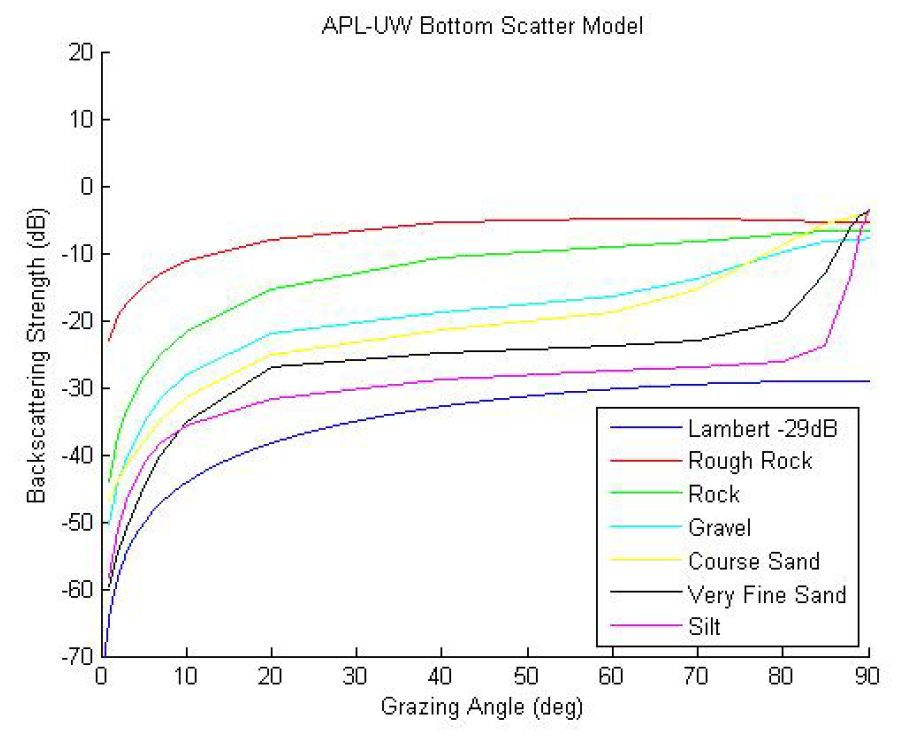
\includegraphics[width=0.8\textwidth]{Chap2/fig/materials}
	\caption{Materials reflective characteristics from \citet{miller2015real}.}
	\label{fig:materials}
\end{figure}
